\documentclass{astroedu-lab}

\begin{document}

\pagestyle{plain}

\begin{problem}{\huge Лабораторная работа 4.4.3\\\\Изучение призмы с помощью\\\\гониометра\\\\Выполнил Жданов Елисей Б01-205}

\section{Цель работы:}

Знакомство с работой и настройкой гониометра Г5

Определение зависимости показателя преломления стекла призмы от
длины волны

Определение марки стекла и спектральных характеристик призмы

\section{Оборудование:}

Гониометр

Ртутная лампа

Призма

Стеклянная плоскопараллельная пластинка

Призменный уголковый отражатель

\section{Теоретическая справка}

Гониометр служит для точного измерения углов и находит широкое применение в оптических лабораториях. С помощью гониометра можно определять показатели преломления и преломляющие углы призм и кристаллов, исследовать параметры дифракционных решёток, измерять длины волн спектральных линий и т. д. В настоящей работе прибор применяется для исследования дисперсии стеклянных призм --- зависимости показателя преломления от длины волны.

	\begin{figure}[h]
		\begin{center}
			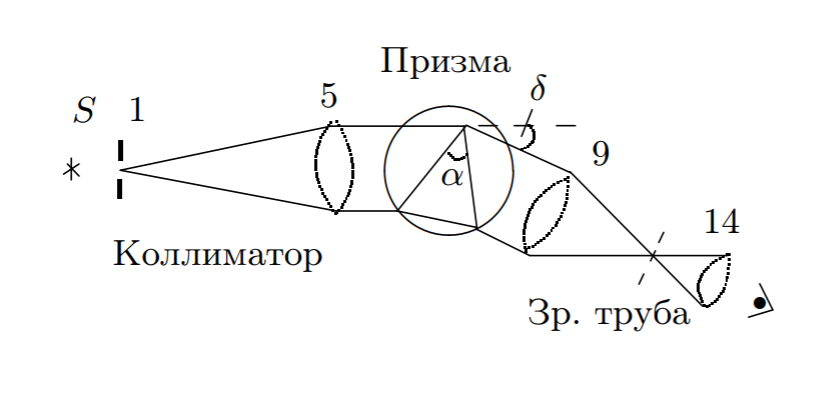
\includegraphics[width = 0.55\textwidth]{443-1.png}
			\caption{Оптическая схема эксперимента}
		\end{center}
	\end{figure}

Показатель преломления материала призмы удобно определять по углу наименьшего отклонения. Известно, что минимальное отклонение луча, преломленного призмой, от направления луча, падающего на призму, получается при симметричном ходе луча (в призме луч идёт перпендикулярно биссектрисе преломляющего угла). Угол минимального отклонения $\delta$, преломляющий угол $\alpha$ (угол при вершине призмы на рис. 1) и показатель преломления $n$ связаны между собой соотношением

\begin{equation}
	n=\dfrac{\sin\dfrac{\alpha+\delta}{2}}{\sin\dfrac{\alpha}{2}}.
\end{equation}

Измерив с помощью гониометра преломляющий угол призмы и углы наименьшего отклонения для света разных длин волн, можно рассчитать величину $n$ и построить дисперсионную кривую --- график зависимости $n(\lambda)$. 
	
По наклону дисперсионной кривой можно оценить разрешающую
	способность призмы
	\begin{equation}
	R = \dfrac{\lambda}{\delta\lambda} = b\dfrac{dn}{d\lambda}.
	\end{equation}
	Здесь $\delta\lambda$ --- минимальный интервал длин волн, разрешаемый по критерию Релея, $b$ --- размер основания призмы, если вся рабочая грань призмы освещена параллельным пучком.

\section{Измерения, Обработка}

1) Откалибруем зрительную трубу, предметный столик, колимматор, входную щель, начало отсчета.

2) Измерим преломляющий угол

Углы, соответствующие отражению колимматорного креста:

$\alpha_1 = 1^\circ 20' 27"$

$\alpha_2 = 118^\circ 21' 59"$

$\Delta \alpha = 117^\circ 1' 32"$

Тогда преломляющий угол $\phi = 62^\circ 58' 28"$

3) Показатели преломления посчитаем по формуле



используя минимальные углы отклонения, полученные при замере призмы

\begin{center}
\begin{tabular}{|c|c|c|c|c|c|c|c|}
\hline 
№ & $K_1$ & 1 & 2 & 3 & 4 & 5 & 6 \\
\hline
$\lambda$, нм & 623.4 & 579.1 & 577.0 & 546.1 & 491.6 & 435.8 & 404.7 \\
\hline
n & 1,6587 & 1,6623 & 1,6625 & 1,6657 & 1,6729 & 1,6838 & 1,6925 \\
\hline
\end{tabular}
\end{center}

Случайная погрешность составляет 1", что намного меньше приборной погрешности, которая может составлять вплоть до 10". Тогда погрешность n составит около $10^{-4}$. Таким значением и определим точность полученных значений n.

Построим дисперсионную кривую

	\begin{figure}[h]
		\begin{center}
			\includegraphics[width = 1\textwidth]{п1.png}
			\caption{Дисперсионная кривая}
		\end{center}
	\end{figure}

Найдем угловые коэффициенты прямых для каждой установки по МНК.

\[
	a = \frac{<x_i y_i> - < x > < y_i >}{< x_i^2> - < x_i >^2}
\]

\[
	b = < \nu_i > - a < N_i >
\]

Также рассчитаем их погрешности

\begin{equation}
	S_a^2 = \frac{< x_i^2>}{< x_i^2 > - < x_i >^2} \cdot \frac{<  b_i - b > ^2}{n - 2}
\end{equation}

Полученная аппроксимация

\begin{equation}
	 n = (1.6949 \pm 0.0066) - (0.000148 \pm 0.000013) \cdot \lambda
\end{equation}

Средняя дисперсия

\begin{equation}
	 \frac{d n}{d \lambda} = 1.50 \cdot 10^3 \pm 2 \cdot 10^2 \text{см}^{-1}
\end{equation}
	
Что соотвествует тяжелому флинту ТФ1.

3) Дисперсия решетки в 1 порядке

\begin{equation}
	 D = 100 \text{ штр/мм} = 10^4 {}^\circ / \text{ нм}
\end{equation}

Дисперсия призмы составит(из МНК для зависимости угла от длины волны) $d \phi/d \lambda = 0.0167 {}^\circ / \text{ нм}$. 

4) По наклону кривой n($\lambda$) рассчитаем максимальную разрешающую способность призмы

\begin{equation}
	 R = a \frac{d n}{d \lambda} = 1100 \pm 100
\end{equation}

По измерениям желтого дублета

\begin{equation}
	 R > \frac{\lambda}{\delta \lambda} \approx 1100
\end{equation}

Оценим, при каком размере решетки 100 штр/мм, она обладает такой же разрешающей способностью как призма с основанием 5 см.

$a \cdot 100 = R = b \frac{d n}{d \lambda}$

$a = 37 \pm 3$ мм

%\begin{figure}[!h]
%	\centering
%	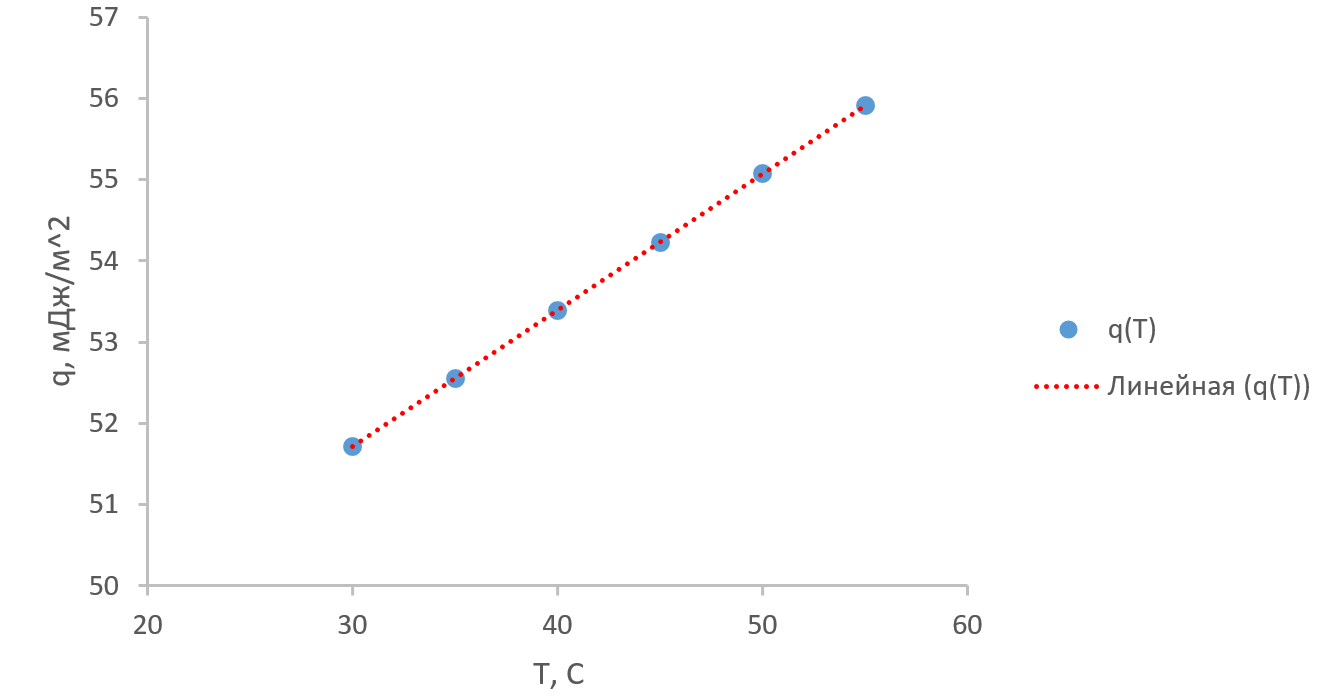
\includegraphics[width=1\textwidth]{2023-02-23_22-23-59.png}
%	\label{fig:boiler}
%\end{figure}

\section{Вывод}

Даже с учетом дисперсии стекла, с помощью призмы удается заниматься довольно точной спектрометрией, если помнить про границы выбранных приближений.


\section{Ресурсы}

Расчет по МНК: метод-наименьших-квадратов.рф


\end{problem}
\end{document}